% \begin{otherlanguage}{english}
%
% % \title{An apportionment method for the Oxidative Potential to the atmospheric PM
% % sources: application to a one-year study in Chamonix, France.}
% %
% %
% % % \Author[affil]{given_name}{surname}
% %
% % \Author[1]{Weber}{Samu\"{e}l}
% % \Author[1]{Uzu}{Ga\"{e}lle}
% % \Author[1]{Calas}{Aude}
% % \Author[1,2]{Chevrier}{Florie}
% % \Author[2]{Besombes}{Jean-Luc}
% % \Author[1,3]{Charron}{Aur\'{e}lie}
% % \Author[1]{Salameh}{Dalia}
% % \Author[4]{Je\v{z}ek}{Irena}
% % \Author[4,5]{Mo\v{c}nik}{Gri\v{s}a}
% % \Author[1]{Jaffrezo}{Jean-Luc}
% %
% % \affil[1]{Univ. Grenoble Alpes, CNRS, IRD, IGE (UMR 5001), F-38000 Grenoble, France.}
% % \affil[2]{Univ. Savoie Mont-Blanc, LCME, F-73 000 Chamb\'{e}ry, France.}
% % \affil[3]{IFFSTAAR, F-69675 Bron, France.}
% % \affil[4]{Aerosol d.o.o., Kamni\v{s}ka 41, 1000 Ljubljana, Slovenia.}
% % \affil[5]{Jo\v{z}ef Stefan Institute, Jamova 39, SI-1000 Ljubljana, Slovenia.}
%
%
% % \begin{abstract}
% % Inhaled aerosolized particulate matter (PM) induces cellular oxidative stress in
% % vivo, leading to adverse health outcomes. The oxidative potential (OP) of PM
% % appears to be a more relevant proxy of the health impact of the aerosol rather
% % than the total mass concentration. However, the relative contributions of the
% % aerosol sources to the OP are still poorly known. In order to better quantify
% % the impact of different PM sources, we sampled aerosols in a French city for one
% % year (year 2014, 115 samples). A coupled analysis with detailed chemical
% % speciation (more than 100 species, including organic and carbonaceous compounds,
% % ions, metals and Aethalometer measurements) and two OP assays (ascorbic acid
% % (AA) and dithiothreitiol (DTT)) in a simulated lung fluid (SLF) were performed
% % in these samples. We present in this study a statistical framework using a
% % coupled approach with Positive Matrix Factorization (PMF) and multiple linear
% % regression to attribute a redox-activity to PM sources. Our results highlight
% % the importance of the biomass burning and vehicular sources to explain the
% % observed OP for both assays. In general, we see a different contribution of the
% % sources when considering the OP AA, OP DTT or the mass of the
% % PM\textsubscript{10}.  Moreover, significant differences are observed between
% % the DTT and AA tests which emphasized chemical specificities of the two tests
% % and the need of a standardized approach for the future studies on
% % epidemiology or toxicology of the PM.
% % \end{abstract}
%
%
% \section{Introduction}  %% \introduction[modified heading if necessary]
% Exposure of the population to pollution by airborne particles is a growing
% concern due to its burden on human health, ranking as the 5\textsuperscript{th}
% risk factor for total deaths from all causes across ages and sexes in 2015
% \parencite{cohenEstimates2017}. Such impact is assessed through cross-over studies
% based on health data and particulate matter (PM) mass concentrations
% \parencite{popeiiiAir2004,popeiiiEpidemiology1999,worldhealthorganizationAmbient2016}. However,
% the dominant fraction of the PM mass are ionic species or crustal elements and
% these contribute little to PM toxicity \parencite{ayresEvaluating2008}.
% Therefore, new metrics are currently investigated in order to better quantify
% the effect of the population exposure. Among the different metrics, oxidative
% potential (OP) addresses the intrinsic capacity of PM to generate Reactive
% Oxygen Species (ROS) able to oxidize the lungs. It has been proposed as a
% unifying factor for quantifying the effects of particulate exposure as it relies
% on surface area, size and PM composition
% \parencite{ayresEvaluating2008,sauvainDifferentiated2009,kellySize2012,gehlingEnvironmentally2013,sauvainComparison2013,fangOxidative2016,crobedduOxidative2017,abramsAssociations2017}.
%
% Many methodologies to quantify OP exist, and none has become a standard so far.
% Since each OP methodology is somewhat specific to the precise type of ROS or
% ROS-inducer \parencite{yangMeasurement2014}, a standard methodology should most
% probably include several assays in order to fully determine the ROS generation
% propensity \parencite{janssenAssociations2015,sauvainComparison2013}. Such a
% combination has not emerged yet, since the link between OP and chemical
% composition of PM is not fully understood, and OP drivers are not truly
% supported by evidence.
%
% Investigating the link between OP and chemistry of PM is not simple, since
% particles chemical composition is unique in every sampling point.  Moreover,
% univariate correlations can lead to false resultsr. For example, strong OP
% correlation with polycyclic aromatic hydrocarbon (PAH) can be found within
% dithiothreitol (DTT) assay \parencite{calasComparison2018}. This correlation is
% chemically impossible since DTT, a reducing agent, needs redox-active compounds
% to be depleted \parencite{ntziachristosRelationship2007,shirmohammadiFine2016}.
% This correlation is now well explained since PAHs are co-emitted with quinones,
% oxy-PAH which are redox-active and able to oxidize DTT
% \parencite{charrierOxidant2015,charrierDithiothreitol2012}. Linear multiple
% regression is not trivial to use in determining OP factors, since extreme
% outliers need to be removed, normal distributions are needed and negative
% contributions may be attributed to mathematically explain annual OP variations
% \parencite{calasComparison2018}.
%
% Another option is to consider the sources contribution instead of the chemical
% species~\parencite{vermaReactive2014,batesReactive2015,fangPM22015,fangOxidative2016}.
% Indeed, working directly with chemical species involves assessing an exhaustive
% composition characterization. This is rather impossible since many species in
% the complex mixture of aerosols remain unidentified. Moreover, if a detailed
% composition (which can sometimes include up to 150
% species~\parencite{wakedSource2014}) is provided, at least the same number of
% samples for OP measurements is needed, otherwise, the system remains
% underdetermined. Reducing the system by direct truncation is not possible since
% species contributing to OP could be dropped, inducing some degree of unknown
% bias. Conversely, if the explanatory variables are the sources’ contributions,
% biases are mitigated.  However, the sources dynamics need to be determined for a
% long period of time in order to reflect the climatology of the location.
% Moreover, the composition of a given named source may vary according to its
% location~\parencite{belisCritical2013}.
% To mitigate theses issues, we decide to use a PMF approach instead of a CMB
% model to better render the local specificities of the sources. Indeed, the CMB
% averages the sources profile’s from different studies and is then locally biased.
% Furthermore, in this study a whole year of analysis is used as input of the PMF.
% We then have a climatological view of the sources dynamics.
%
% The objective of this study is to present a methodology for the evaluation of
% the contributions of common sources of particles to the overall OP for a long
% time series of PM\textsubscript{10} sample (PM with a diameter lower than
% \SI{10}{\micro\meter}). The OP was measured on filter samples collected
% over a full year in the city of Chamonix (Alpine valley), using two OP
% protocols: the ascorbic acid (AA) and dithiothreitol (DTT) assays. An inversion
% procedure of these OP measurements was developed using source apportionment
% results obtained from an advanced source-receptor model PMF
% \parencite{chevrierChauffage2016}, in order to attribute both an intrinsic OP to
% the sources and the evolution of the sources contributions to OP's over
% the year.
%
%
% \section{Methods}
%
% This work takes advantage of an already existing database, based on Particulate
% Matter (PM\textsubscript{10}) samples collected during the DECOMBIO program
% \parencite{chevrier_decombio-contribution_2016}, with the chemical analyses and the
% source apportionment of PM having already been conducted
% \parencite{chevrierChauffage2016}, and the OP measurements performed on the
% same samples \parencite{calasComparison2018}.  These are briefly presented below.
%
%
% \subsection{Site and sampling}\label{site-and-sampling}
%
% Sampling took place in the city of Chamonix-Mont-Blanc
% (\ang{45;55.358;}~N, \ang{6;52.194;}~E),
% in the Alpine Arve Valley, below Mont-Blanc (Figure~\ref{fig:cham}). The
% sampling site is located in the middle of the town, in a densely populated area,
% with the sampling cabin being close to a street. A one-year study was conducted
% from November, 14\textsuperscript{th} 2013 to October, 31\textsuperscript{th}
% 2014, with 24 hour PM\textsubscript{10} sampling taking place every third day,
% giving a series of 115 samples. These daily PM\textsubscript{10} samples were
% collected with a high volume sampler (Digitel, DA80, \SI{30}{\cubic\meter\per\hour}) on
% pre-fired quartz filters (Pall, Tissuquartz). All details concerning the site
% and the logistical aspects of the sampling procedure can be found in
% \textcite{chevrierChauffage2016}.
%
% \begin{figure}[ht]
%     \centering
%     \includegraphics[width=8.3cm]{chapter04/fig01.png}
%     \caption{Location of the sampling site in Chamonix, in the Arve Valley,
%     France (\ang{45;55.358;}~N, \ang{6;52.194;}~E).  $\copyright$~Planete observer, IGN}
%     \label{fig:cham}
% \end{figure}
%
% \subsection{Chemical analyses }\label{chemical-analyses}
%
% All filters were analyzed using a large array of methods for the quantification
% of chemical species including those important for the mass balance of the PM
% (EC, OC, ions\ldots{}) and many organic and inorganic tracers of
% sources. The elements and components analyzed are:
%
% \begin{itemize}
% \item
%   Organic and elemental carbon (OC, EC), using a Sunset instrument and
%   the EUSAAR2 protocol \parencite{aymozEvolution2004,cavalliEuropean2016};
% \item
%   soluble anions and cations (NO\textsubscript{3}\textsuperscript{-},
%   SO\textsubscript{4}\textsuperscript{2-}, Cl\textsuperscript{-} and
%   NH\textsubscript{4}\textsuperscript{+}, Mg\textsuperscript{2+},
%   Na\textsuperscript{+}, Ca\textsuperscript{2+}, K\textsuperscript{+})
%   through ionic chromatography \parencite{wakedSource2014};
% \item
%   inorganic elements (Al, Fe, Ti, As, Ba Cd, Ce, Cr, Cu, La, Li, Mn, Mo,
%   Ni, Pb, Rb, Sb, Sn, Sr, V, Zn and Zr) using ICP-MS \parencite{wakedSource2014};
% \item
%   sugar alcohols (arabitol, sorbitol, and mannitol, also called polyols)
%   and anhydrous monosaccharides (levoglucosan, mannosan and galactosan)
%   using an HPLC-PAD method \parencite{wakedSource2014};
% \item
%   polar and nonpolar organic tracers (alkanes, hopanes, methoxyphenols,
%   and substituted derivatives (methyl-PAHs) and polycyclic aromatic
%   sulfur heterocycles (PASHs) using GC-MS and polycyclic aromatic
%   hydrocarbons (PAHs) using HPLC-fluorescence \parencite{gollyLarge2015}.
% \end{itemize}
%
% Additionally, Black Carbon (BC) measurements were ongoing throughout the year,
% with wood burning BC\textsubscript{bb} and fossil fuel BC\textsubscript{ff}
% fractions determined using an Athalometer AE33 and the so called ``Aethalometer
% model'' \parencite{sandradewiUsing2008,drinovecDualspot2015}.  Although the BC
% measurements was performed on PM\textsubscript{2.5} samples, we decided to use
% it as \textcite{jaffrezoSize2005,cavalliEuropean2016} show that the amount of EC in
% PM\textsubscript{10} and PM\textsubscript{2.5} is almost equivalent.
%
% All the procedures for these chemical analyses
% are described in detail in \textcite{chevrierChauffage2016}.
%
% \subsection{\texorpdfstring{Source apportionment of PM\textsubscript{10}}{Source
% apportionment of PM10}}\label{source-apportionment-of-pm10}
%
% The source apportionment was performed with Positive Matrix Factorization, using
% the US EPA software PMF 5.0 \parencite{usepaPositive2017}, following the
% recommendations included in the european guideline book issued in the EU Fairmode program
% \parencite{belisEuropean2014}. However, in the environment of Alpine valleys, the
% local meteorology and frequent inversion layers in winter lead to strong
% covariations of the concentrations of many chemical species emitted from the
% valley bottom.
% Indeed, during temperature inversion in Alpine valley, pollutants are stuck into
% the Atmospheric Boundary Layer (ABL) and cannot be removed by wind. Such
% inversion may be stable during several days. As a result, the different emission
% sources during that period of time add together and the dynamic from the
% different sources is masked. In other words, one sample does not integrate
% anymore only emissions during the sampling time, but also emissions of the
% previous days. This end-up with chemical species in one sample that should not
% be present together, respect to the temporality of their respective sources.
% Thereby, their correlation is increased.
% The covariation of the different pollutants adversely influences the ability of
% PMF to distinguish different sources.
% Therefore, we developed an approach including several specificities, rarely
% applied in classic source apportionment, in order to overcome this
% methodological problem in the PMF \parencite{chevrierChauffage2016}.
%
% First, many tracers were included as input parameters, including specific
% organic tracers. The benefit of such approach was previously described
% \parencite{gollyEtude2014,wakedSource2014,srivastavaSpeciation2017}. In our
% case, we included hopanes (thereafter named HOP), methoxyphenols, polyols (sum
% of mannitol, arabitol and sorbitol), levoglucosan and MSA (methane sulfonic
% acid). Instead of OC we used the difference (OC*) between the OC and
% the carbon equivalent of these previously analyzed species.
%
% Second, elemental carbon (EC), which is an important species for the
% deconvolution of combustion sources was in the PMF replaced by
% BC\textsubscript{bb} and BC\textsubscript{ff} obtained using the ``Aethalometer
% model'' by concurrent measurements with the Aethalometer AE33. This provides a
% very strong information on the sources, as already pointed out in other studies
% \parencite{petitTwo2015}. No correction was introduced to compensate between EC
% and BC \parencite{zanattaEuropean2016}.
%
% Finally, we took advantage of the possibilities of PMF 5.0 to apply
% constraints to the factor profiles, in order to better define the sources
% \parencite{gollyEtude2014,srivastavaSpeciation2017,salamehImpacts2015}.
% A minimal set of constraints based on prior and external geochemical knowledge
% of sources fingerprints was applied:
% \begin{itemize}
%     \item
%         in the biomass burning factor, the contributions of levoglucosan, potassium,
%         methoxyphenols and BC\textsubscript{bb} were increased,
%         whereas the BC\textsubscript{ff} and HOP were set to 0,
%     \item
%         HOP was increased in the vehicular factor.
% \end{itemize}
% We increased the concentration of the species in the factors thanks to the “pull
% up maximally” option of the EPA PMF5.0 software~\parencite{usepaPositive2017},
% which tried to increase the contribution of the given specie to the factor.
% Table~\ref{tab:PMFentry} sums up the input chemistry species and respective uncertainties
% used in the PMF study.
% \begin{table*}
%     \centering
%     \caption{Selection of the chemical species used as input variables in the EPA PMF5.0
%         model and their relative uncertainties. $\Sigma$polyols refers to the sum of
%         arabitol, sorbitol and mannitol and $\Sigma$methoxyphenol to the sum of the
%         particulate methoxyphenols.  The uncertainties in ``\%'' are relative to
%         the sample concentration for the species.}
%         \scriptsize
%     \begin{tabularx}{\textwidth}{Xlccm{2.7cm}m{1.5cm}m{2.6cm}m{3cm}}
%         \toprule
%         & Total & \multicolumn{2}{c}{Carbonaceous matter} & Ions &
%         \multicolumn{2}{c}{Organics compound} & Metals\\
%         \midrule
%         Species & PM\textsubscript{10} & OC* &
%         BC\textsubscript{bb}, BC\textsubscript{ff} & Cl\textsuperscript{-},
%         NO\textsubscript{3}\textsuperscript{-},
%         SO\textsubscript{4}\textsuperscript{2-}, Na\textsuperscript{+},
%         NH\textsubscript{4}\textsuperscript{+}, K\textsuperscript{+},
%         Mg\textsuperscript{2+}, Ca\textsuperscript{2+} &
%         $\Sigma$polyols, MSA,\newline levoglucosan &
%         $\Sigma$HOP, $\Sigma$Methoxyphenol &
%         As, Cu, Fe, Mn, Mo, Ni, Pb, Rb, Sb, Ti, V, Zn, Zr
%         \\
%         Uncertainty & 20\% & 10\% & 20\% & \textcite{gianiniSource2013} & 15\% &
%         \textcite{gianiniSource2013} & 2$\times$\textcite{gianiniSource2013} \\
%         \bottomrule
%     \end{tabularx}
%     \label{tab:PMFentry}
% \end{table*}
%
%
% \subsection{Measurements of the Oxidative Potential of PM}
% \label{measurements-of-the-oxidative-potential-of-pm}
%
% The methodology is described in detail in \textcite{calasImportance2017}. In
% brief, we performed the extraction of PM into the simulated lung fluid (SLF)
% solution to simulate the bio-accessibility of PM and to closer simulate
% exposure conditions. The extraction took place into SLF at iso-mass. All samples
% were analyzed at \SI{10}{\micro\g\per\milli\liter} of PM, by adjusting the area of filter
% extracted.
% The filter extraction method includes both water soluble and insoluble species.
% After the SLF extraction, particles removed from filter are not filtrated; the
% whole extract is injected in the multiwall plate.  
% Samples were processed using the AA and DTT assays. DTT depletion when in
% contact with PM extracts was determined by dosing the remaining amount of DTT
% with DTNB (dithionitrobenzoic acid) at different reaction times and absorbance
% was measured at \SI{412}{\nano\meter} using a plate spectrophotometer (Tecan, M200). The
% AA assay is a simplified version of the synthetic respiratory tract lining fluid
% (RTFL) assay \parencite{kellyProtein2003}, where only AA is used. AA depletion is
% read continuously for \SI{30}{\min} from absorbance at \SI{265}{\nano\meter} (TECAN,
% 200). 
% The maximum depletion rate of AA is determined by linear regression of the
% linear section data. 
%
% Both reaction have a non-linear cinetic. However, the two reactants (DTT and AA)
% are in large exces. We then measure the depletion rate in first part of the
% reaction, which can be estimated by a linear reaction (in the first 20 to 30
% minutes).
%
% For both assays, the 96-wells plate is auto shaken for 3
% seconds before each measurement and kept at \SI{37}{\degreeCelsius}.  Three filter
% blanks (laboratory blanks) are included in every plate (OP AA and OP DTT) of the
% protocol. The average values of these blanks are then subtracted from the sample
% measurement of this plate. LOD value is defined as three times of the standard
% deviation of laboratory blanks measurements (blank filters in Gamble+DPPC
% solution).
%
% The samples were stored 3 years before analyzed. As mentioned
% in~\textcite{vermaOrganic2015}, the OP activity may be impacted by such storage
% time. However, in a previous program \parencite{ansesexposureEtude2017}, still
% ongoing, we have been measuring the same filter over time.  After one year, OP
% results for AA assay remain equivalents. DTT results showed a regular decrease
% of 15~\% the first 6 months before stabilization. 
%
% Only 98 samples out of the 115 collected were measured for OP, removing samples
% with insufficient PM mass concentration (\SI{<5}{\ugm}) that
% did not afford filter extraction at \SI{10}{\micro\g\per\milli\liter}. The oxidative
% potential (OP) unit is then expressed in nmol per minute per microgram of PM.
% However, the population exposition is (in the first order) proportional to the
% mass of the inhaled PM. Therefore, the OP per microgram was multiplied by the
% total mass concentration of PM (\si{\ugm}) in order to express the OP
% in unit of~\si{\opv}. We should however keep in mind that this
% measurement of OP may not be the exact OP from PM inhaled by the population,
% since we suppose a linear relationship between the OP per~\si{\micro\g} of PM and
% the OP of the total amount of PM. Indeed, some cocktail effects like
% complexation or chelation may occur for PM concentrations higher than the one
% tested. It has been shown by \textcite{calasImportance2017} that the result is
% generally a probable over-estimation of the ``true'' OP. Hereafter, the OP
% normalized by volume is denoted with a subscribed v (OP AA\textsubscript{v} and
% OP DTT\textsubscript{v}).
%
% \section{Results}\label{results}
%
% \subsection{Evolution of the OP}\label{evolution-of-the-op}
%
% Both assays present a strong seasonality (Fig.~\ref{fig:OPts}) as already
% mentioned in \textcite{calasImportance2017}, and both the OP AA\textsubscript{v}
% and OP DTT\textsubscript{v} results show seasonality. The OP\textsubscript{v}
% remains high during winter and low during summer.  This observation tends to
% emphasize the importance of PM sources which also show distinct seasonality.
% However, we can also observe fast variations from day to day, which may be
% related to a change in the PM chemistry or composition or a change in PM concentration
% related to sources or meteorological conditions.
%
% Despite both assays following the same annual trend, some significant
% differences exist. For instance, during summer, OP DTT\textsubscript{v} shows
% larger values, whereas the values of OP AA\textsubscript{v} are close to 0.
% Moreover, the variation of the OP AA\textsubscript{v} seems smoother than that
% of OP DTT\textsubscript{v}, especially during summer and fall (May to November). 
% This underlines that the assays are sensitive to different chemical species
% present in PM.
%
% \begin{figure}[ht]
%     \centering
%     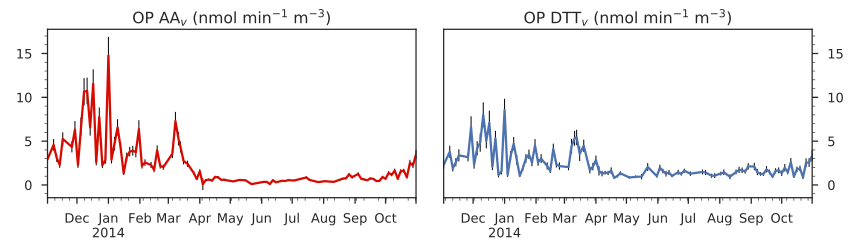
\includegraphics[width=\textwidth]{chapter04/fig02}
%     \caption{OP AA\textsubscript{v} and OP DTT\textsubscript{v} variation from
%         2 November 2013 to 31 October 2014 (98 samples) at the Chamonix
%         station. The error bars represent the uncertainties (standard
%         deviation) of the measurement. The OP unit is normalized by volume and
%         is expressed in~\si{\opv}.  }
%     \label{fig:OPts}
% \end{figure}
%
% \subsection{Evolution of the sources contributions}\label{evolution-of-the-sources-contributions}
%
% The PMF was already thoroughly discussed in~\textcite{chevrierChauffage2016}.
% Briefly, 8 sources were identified: biomass burning, crustal dust, nitrate rich,
% sulfate rich, primary biogenic emissions an secondary biogenic aerosol, salt and
% vehicular emissions. Their respective main chemical species and related
% information are provided in the Supplementary Information (SI 1). We mainly see
% that metals (notably copper) and some organics species are highly correlated to
% both OP, together with many fractions of the carbonaceous matter (OC,
% BC\textsubscript{bb} and BC\textsubscript{ff}, see SI 2).
% Figure~\ref{fig:PMFsrc} presents sources contributions to PM. The dominant PM
% source is biomass burning during winter with some daily concentrations exceeding
% \SI{40}{\ugm}. The primary and secondary biogenic sources are mainly
% active during summer, as is the sulfate rich source. The vehicular source is
% quite constant all over the year. Indeed, the higher concentration during
% winter may be attributed to accumulation in the ABL, and not to an increase of
% emission. The crustal dust contribution is sporadic and
% could include some Saharan episodes \parencite{aymozEvolution2004}. Finally, the
% salt source is low but presents a high spike during March, being maybe related
% to road salting at that time of the year. The correlation between the OP and the
% sources are presented and discussed in the SI 2. 
% Briefly, the vehicular and biomass burning sources appear to be strongly
% correlated to both OP ($r>0.8$). The nitrate-rich factor presents a lower
% correlation, as well as the sea/road salt one ($0.3<r<0.6$ for both OP’s),
% whereas the secondary biogenic, primary biogenic, and sulfate-rich factors are
% slightly anti correlated with both OP’s ($‑0.6<r<‑0.3$). Crustal dust
% correlation is not significant with respect to the AA test but presents low
% correlation to the DTT test ($r=0.15$ and $r=0.35$, respectively).
%
% \begin{figure}[ht]
%     \centering
%     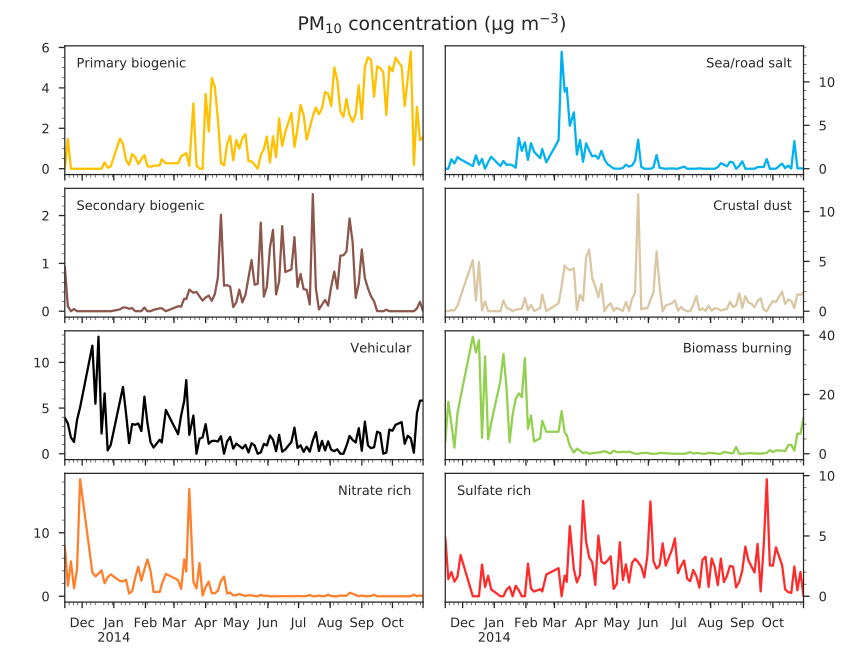
\includegraphics[width=\textwidth]{chapter04/fig03}
%     \caption{Mass concentrations of the eight PMF sources as fractions of PM\textsubscript{10} from 14 November 2013 to 31 October 2014 (107 samples)
%     at the Chamonix station. Units are expressed in~\si{\ugm}. Note
% different scales on the source contributions.  }
%     \label{fig:PMFsrc}
% \end{figure}
%
% \subsection{Setting up a multiple linear regression}
% \label{setting-up-a-multiple-linear-regression}
%
% As the OP is a value of reactivity, it cannot be directly introduced in
% a mass-balance model. Hence, in order to estimate the contributions of
% the PM sources to the OP, we must use an inversion
% method. Despite the possible non linearity of OP values with increasing
% masses of PM, as discussed below, we assume in this work that the OP is
% linearly linked to the mass. Thus, we hereafter assume that OP and the
% explanatory variables, namely the mass of the PM sources
% m\textsubscript{PM}, are linearly related as follows
% \begin{equation}
%     \text{OP}_{\text{obs}} = m_{\text{PM}} \cdot \beta + \varepsilon
%     \label{eq:sys}
% \end{equation}
% where OP\textsubscript{obs} is the ($n\times1$) observed OP matrix in~\si{\opv}, m\textsubscript{PM} the ($n\times(p+1)$)
% matrix with the PM mass attributed to each source expressed in~\si{\ugm} and a constant unity term with no unit
% for the intercept, and $\varepsilon$ the ($n\times1$) uncertainty matrix
% in~\si{\opv}; n is the number of samples and
% p the number of sources. The estimator $\beta$ (matrix $(p+1)\times1$) represents
% the intrinsic OP of the sources (i.e. the OP per mass unit of PM
% attributed to a given source) and the intercept, expressed respectively
% in~\si{\opm} for the intrinsic OP and in~\si{\opv} for the intercept.
%
% The optimal approximation of a solution for the linear system expressed
% by equation \ref{eq:sys} is typically found by least squares. A variety of
% methods exist differing on the function to be minimized and on the
% regularization or sparsity penalty imposed to perform variable selection
% on $\beta$, from ordinary least squares to ridge regression and LASSO (least
% absolute shrinkage and selection operator). Here we have chosen a
% Weighted Least Squares (WLS) approach as it has an integrated way to
% handle the OP uncertainties. We have also chosen not to add a penalty
% function as we do not have prior knowledge on the intrinsic OP values.
% However, regular WLS do not rule out negative solutions, which should be
% implemented in our case since it is not demonstrated that intrinsic OP
% negative values exist in the real world. Therefore, a stepwise
% regression is conducted. The underlying algorithm is
%
% \begin{enumerate}
%     \item
%         Solve the WLS problem and estimate the intrinsic OP,
%     \item
%         If an intrinsic OP is negative, then set it to zero and go back to step
%         1,
%     \item
%         Repeat until all intrinsic OPs are positive or zero.
% \end{enumerate}
%
% No source is discarded based on its p-value but only if its intrinsic OP
% is negative. We did not choose a direct non-negative least square
% approach as it would be a constraint in the model we believe is too strong. In addition,
% we can use the absence of negative coefficients as a test for the
% coherence of our dataset. Such approach may allow us to
% investigate which sources present a negative OP and why. This loop
% converges in a finite number of iterations, either to a situation with
% zero sources -- which would be discarded as absurd, pointing to a
% breakdown of the underlying assumptions, or to an acceptable solution
% with a lower number of sources. In our particular case, since OP
% measurements never display negative values or negative source
% contributions from the PMF, the method is strictly guaranteed to
% converge to an acceptable solution. Further, we expressly do not set the
% intercept to zero in Eq.~\ref{eq:sys}, choosing instead to use this as a
% check on our method. If the system is well constrained (i.e. no
% missing sources) the intercept should be close to zero within the model
% uncertainties, without any explicit constraint. The reciprocal situation
% could point to missing explanatory variables.
%
% The uncertainties of the intrinsic OP are extracted from the variance of
% $\beta$, which in turn is derived from the Hessian matrix of the WLS
% regression in the standard way. However, the uncertainties on the
% modelled OP are not analytically computed. Indeed, some coefficients
% present co-variation due to the activity of the sources in the very same
% period of the year, so analytical variance cannot be used to estimate
% uncertainties. Therefore, in order to estimate the uncertainties of the
% modelled OP, we bootstrap the solution $\beta$ 1000 times with a Monte-Carlo
% algorithm. The bootstrap simply selects randomly an intrinsic OP for
% each source according to their respective normal distribution.
%
% The algorithm was implemented in Python~3 making use of the
% \emph{statsmodels} WLS module \parencite{seaboldStatsmodels2010}.
%
%
% The method proposed here is an improvement of the one
% of~\textcite{batesReactive2015} and our methods differ in several points.
% First of all, our backward elimination criteria is based on the negativity of a
% source and not in its p-value. Indeed, a source might present a statistically
% significant negative value. But according to us, a source with negative
% intrinsic OP does not have a geo-chemical sense as the air is known to be a
% strong oxidant milieu.
% Secondly, as~\textcite{batesReactive2015} didn’t measure the uncertainty of their
% OP samples, they used an ordinary least square (OLS) regression. On the
% opposite, we have an estimation of our measurements uncertainty thanks to
% triplicate. We then use a weighted least square (WLS) regression instead.
% Finally, we propose a way to estimate uncertainties of our estimated OP with a
% Monte-Carlo method, which is not provided in the previous study.
% Moreover, the method proposed here does not only include the multiple
% linear regression (MLR) but also the use of the PMF model instead of the CMB
% one.  Indeed, the MLR is highly sensitive to the explanatory variable and we
% decide to use the local sources’ profile (PMF) instead of the chemical mass
% balance method with ensemble-averaged source impact profiles.
%
% \subsection{Application to the Chamonix site and
% discussion}\label{application-to-the-chamonix-site-and-discussion}
%
% Figure~\ref{fig:TSobsvsmodel} shows the comparison between observed and modelled
% OPs for the measurements at the Chamonix site for both OP AA and OP DTT assays.
% Table~\ref{tab:OPi} presents the intrinsic OP AA and OP DTT
% in~\si{\opm} for each source with their respective
% uncertainties and p-values.
%
% \subsubsection{Accuracy of the model}\label{accuracy-of-the-model}
%
% The method developed in this study appears to be sufficiently accurate
% to explain the two OP annual series at Chamonix. First, the seasonal
% trend of the OP is very well reproduced, despite some under-estimation
% of some of the highest values in winter. Second, the intercept of the
% equation regression for OP AA\textsubscript{v} is not significant
% (p\textgreater{}0.05). It is not so clear for the DTT test, but the
% p-value remains high (p=0.04). We can consider the intercepts of the
% equation regression as nearly negligible (see Table~\ref{tab:OPi}). The PM sources
% presented in this study are then sufficient to explain the observed OP
% AA\textsubscript{v} and OP DTT\textsubscript{v} time series. We can also
% note that none of the sources was excluded for the DTT assay during the
% inversion procedure due to negative contributions. It emphasizes the
% fact that the sources explain well the observed OP. However, one source
% was discarded for the AA assay: the crustal dust. Its p-value was less
% than~0.01 for an intrinsic OP of \SI{-0.05(1)}{\opm}. We supposed that the
% crustal dust source in this study is a mixing of several sources,
% including Saharan dust and road suspension dust. We could then end-up
% with a mixing of highly different redox-active compounds towards AA test
% that could explain the error for this source. Further work is needed to
% understand this behavior.
%
% \subsubsection{Uncertainties and residual}\label{uncertainties-and-residual}
%
% The uncertainties of the modeled OP are quite low and mostly in the range of the
% measurement uncertainties (Figure~\ref{fig:TSobsvsmodel}). Indeed, the
% distribution of the residual is close to the normal law
% (Figure~\ref{fig:residual}).  However, we can note an asymmetry toward
% underestimation and residual seem to increase almost linearly with the
% endogenous variable (no random repartition around 0 for the highest OP). The OP
% is underestimated by the model for these days featuring concentrations. It may suggest
% either non-linearity with high loading (as suggested above), or particular event
% that is not apportioned by the sources provided in this study.
%
% \begin{figure}[ht]
%     \centering
%     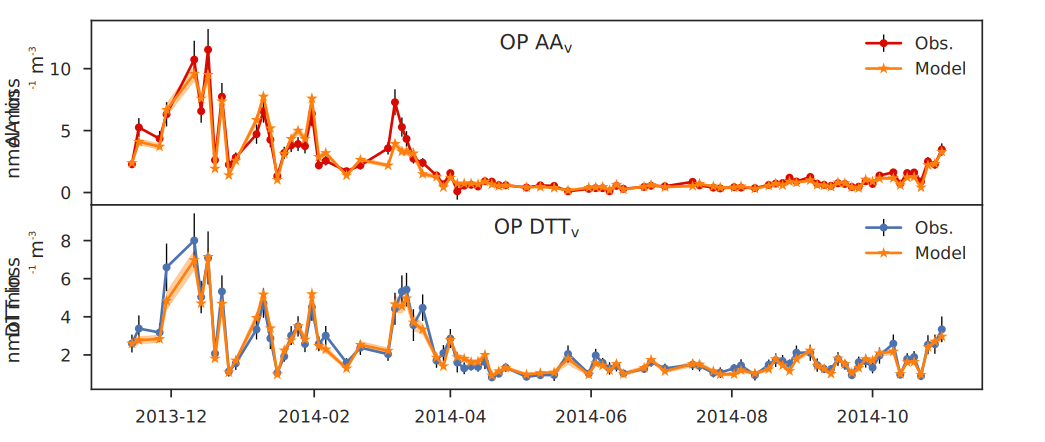
\includegraphics[width=\textwidth]{chapter04/fig04}
%     \caption{Comparison of the modelled OP (orange) and the observed OP for both
%         the AA (top graph) and DTT (bottom graph) test (85 samples) from
%         November 2013 to November 2014. The black error bars are the standard
%         deviation of the observed values and the shaded orange area the
%     uncertainties of the modelled OP.  Units are in OP normalized by volume
%     and expressed in~\si{\opv}.}
%     \label{fig:TSobsvsmodel}
% \end{figure}
%
% \begin{figure}[ht]
%     \centering
%     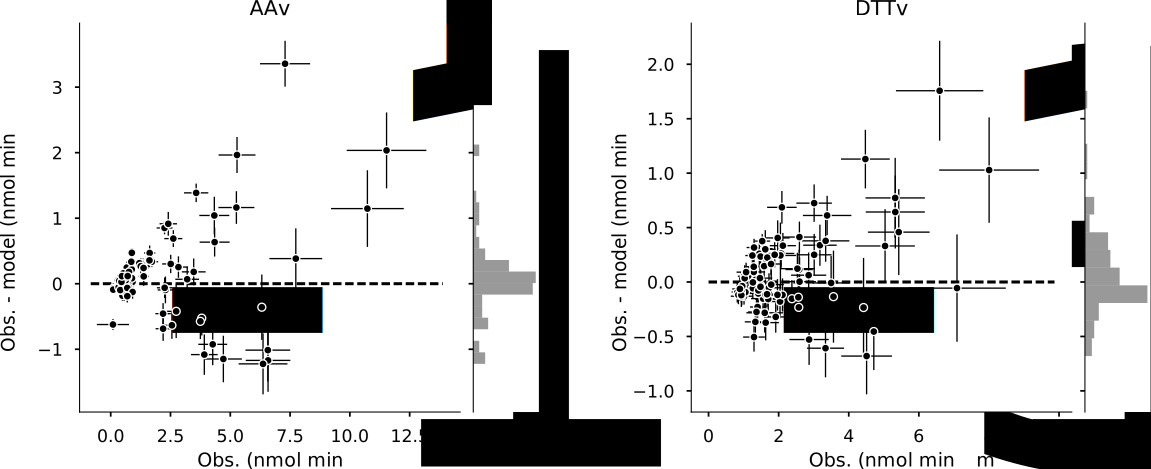
\includegraphics[width=0.9\textwidth]{chapter04/fig05_h}
%     \caption{Residual distribution for the regression of the AA and DTT assays
%         (85 samples). The error bars represent the standard deviation of the
%         observation and the model. The histogram on the right is the
%         distribution of the residuals. Units are in OP normalized by volume and
%         expressed in~\si{\opv}. Note different scales for the
%     AA\textsubscript{v} and the DTT\textsubscript{v}.}
%     \label{fig:residual}
% \end{figure}
%
% \subsubsection{Intrinsic OP}\label{intrinsic-op}
%
% Values of the intrinsic OP of different sources for both the AA and DTT assays are ranging
% from zero to \SI{0.18(1)}{\opm} for the AA test and from \SI{0.06(2)}{\opm} to
% \SI{0.27(3)}{\opm} for the DTT test (Table~\ref{tab:OPi}). The various sources do not
% have the same reactivity toward the AA and DTT. We also note that the two tests present
% different intrinsic OP for the same source, and the relative importance of the sources
% differs from one test to the other. For instance, the vehicular source displays a lower
% intrinsic OP (\SI{0.15}{\opm}) than the biomass burning (\SI{0.18}{\opm}) for the AA test
% but a higher intrinsic OP for the DTT test (\SI{0.27}{\opm} for the vehicular and
% \SI{0.07}{\opm} for the biomass burning).  This deconvolution method may be able to
% account for the chemical specificity of the two OP assays. In addition, the DTT test seems
% to be more multi-sources influenced than the AA test.
%
% Nevertheless, we clearly see the importance of the vehicular source, which is
% associated to a strong intrinsic OP in both the AA and DTT assays. Previous
% studies \parencite{batesReactive2015,fangOxidative2016,vermaReactive2014} also
% highlighted the importance of this source to explain the OP AA and DTT. We may
% explain such high intrinsic OP by the presence of metals in this source
% -- notably the copper \parencite{charrierOxidant2015}.
%
% In the AA assay, the biomass burning also presents a high redox-activity
% per~\si{\micro\g} of PM. This result disagrees with \textcite{fangOxidative2016}
% as they found no activity for this source in the OP AA test. Such difference for
% the biomass burning source may be explained by the two extraction protocols (in
% water or in a SLF solution) or by the proximity of the biomass source in
% Chamonix compared to the longer distance transport in Atlanta, that would change
% the chemistry of the source profile. However, the biomass burning in the OP DTT
% test has an intrinsic OP of \SI{0.07(1)}{\opv}, which is
% coherent with the previous study of \textcite{fangOxidative2016}. The presence of
% oxygenated compounds such as quinones which are redox-active in the organic
% matter could explain this high intrinsic OP.
%
% The nitrate-rich source also appears to contribute in the redox-activity in both
% assays. Although the nitrate itself is not redox-active, it can be present with
% species that are oxidants. More work is needied in order to understand the
% evolution of intrinsic OP for the nitrate rich factor, including measurements on
% series characterized by specific spring events related to agricultural
% activities, and series close to traffic sites for NO\textsubscript{x} emissions.
%
% The primary biogenic source, mainly identified by the presence of polyols,
% presents a significant intrinsic OP. This result was unexpected. Indeed,
% \textcite{liuTherapeutic2010} shows that mannitol is a strong anti-oxidant. Our
% result suggests that some chemical species, present in the primary biogenic
% source but not measured in this study, may contribute to the OP of the PM from
% this source. Recently, it was shown that fungal spores exhibit a significant
% intrinsic OP \parencite{samakeUnexpected2017}, and this may be an hypothesis to be
% further tested. However, the PMF profile of the primary biogenic source may also
% be a mixing of different sources in our study (there is BC\textsubscript{ff} in
% it for instance). Such mixing may also explain the high intrinsic OP of this
% source.
%
% Nevertheless, all these results contrast with those from simple univariate
% correlations between OP and sources. Indeed, the secondary biogenic source which
% is slightly anti-correlated to both OP’s is in fact the second most redox-active
% source when considering intrinsic OP DTT. On the contrary, the sulfate-rich
% factor is slightly anti-correlated to the OP AA\textsubscript{v} but present an
% intrinsic OP AA close to 0. The vehicular factor, which highly correlates with
% OP’s is also the dominant source in terms of intrinsic OP’s for both assays.
% Such results emphasize the real interest to go replace the simple univariate
% correlation by a more comprehensive statistical analysis when considering the
% contribution of the sources (or species) to the OP’s.
%
%
% \begin{table*}
%     \centering
%     \caption{Regression coefficients (i.e. intrinsic OP) expressed
%         in~\si{\opm} at Chamonix for the AA and DTT
%         assays. The values are the mean$\pm$standard deviation based on N=1000
%         bootstrap of the best solution. The p-value is in the parenthesis. The
%         crustal dust source was excluded during the inversion process for the AA test.}
%         \scriptsize
%         \begin{tabularx}{\textwidth}{lXXXXXXXXp{2.2cm}}
%         \toprule
%         & Biomass\newline burning & Crustal\newline dust & Nitrate\newline  rich
%         & Primary\newline biogenic & Sea/road\newline salt & Secondary\newline  biogenic &
%         Sulfate\newline rich & Vehicular & Intercept\\
%         \midrule
%         Unit & \multicolumn{8}{c}{\si{\opm}} & {\si{\opv}}\\
%         \midrule
%         AA & 
%         0.18$\pm$0.01\newline (<0.001) & -\newline (-) &
%         0.12$\pm$0.02\newline (<0.001) & 0.07$\pm$0.01\newline (<0.001) &
%         0.03$\pm$0.01\newline (0.140) & 0.02$\pm$0.04\newline (0.598) &
%         0.00$\pm$0.01\newline (0.942) & 0.15$\pm$0.02\newline (<0.001) &
%         0.05$\pm$0.08\newline (0.502)\\
%         DTT & 
%         0.07$\pm$0.01\newline (<0.001) & 0.07$\pm$0.02\newline (0.003) &
%         0.07$\pm$0.02\newline (<0.001) & 0.12$\pm$0.02\newline (<0.001) &
%         0.14$\pm$0.03\newline (<0.001) & 0.18$\pm$0.05\newline (<0.001) &
%         0.06$\pm$0.02\newline (<0.001) & 0.27$\pm$0.03\newline (<0.001) & 
%         0.17$\pm$0.08\newline (0.045)\\
%         \bottomrule
%     \end{tabularx}
%     \label{tab:OPi}
% \end{table*}
%
% \subsubsection{Contribution to the OP}\label{contribution-to-the-op}
%
% The aim of this study was to establish a deconvolution model for the OP. The
% results obtained with it will be discussed in depth in another study, including
% other sites. However, here are some preliminary results for the Chamonix
% station concerning the sources contribution.
%
% Due to the different intrinsic OP of the sources, the source contributions to
% the OP (intrinsic OP times by the source contribution in~\si{\ugm}) is
% different from their contribution to the PM mass.
% Figure~\ref{fig:contributions} illustrates the normalized contribution of the
% sources to the mass of the aerosols and the OP measures with AA and DTT. It
% shows that the vehicular source barely contributes to 17~\% of the total PM mass
% during March-April-May (MAM) and June-July-August (JJA) but more than 30~\% to
% the OP DTT\textsubscript{v} in the same period, and even reaching around 50~\%
% of the OP AA\textsubscript{v} in JJA. Conversely, some sources largely
% contributing to the PM\textsubscript{10} mass such as the sulfate-rich source
% (30~\% of the total PM mass in JJA) do not contribute to the OP (2~\% to the OP
% AA\textsubscript{v} in the same period). Finally, some sources like the biomass
% burning contribute to a large extend in both PM mass and OP (on an annual basis:
% 35~\% of the PM mass, 55~\% of the OP AA\textsubscript{v} and 22~\% of the OP
% DTT\textsubscript{v}). We also note that on an annual basis, the contribution of
% the vehicular source is much larger for both OP assays than for the mass.  All
% these outcomes are key parameters for policy initiatives.
%
% To sum up, with this methodology, we observe a redistribution of the relative
% importance of the sources ranked as ROS contributors. This study gives, and more
% generally, the OP gives us a new vision of the atmospheric aerosols and
% associated ROS burden. We also point out a clear distinction between the
% different OP tests. Such differences raise new questions on OP assays choices
% and standardization and require further investigation, especially coupled
% OP-toxicology-epidemiology studies.
%
% \begin{figure}[ht]
%     \centering
%     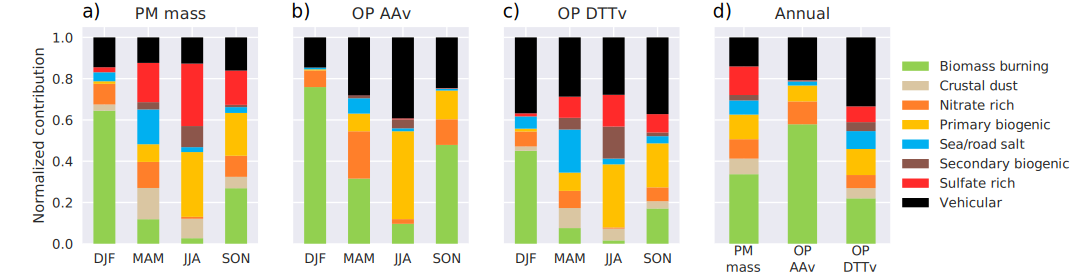
\includegraphics[width=\textwidth]{chapter04/fig06}
%     \caption{Normalized seasonal contribution of the sources to a) the
%     PM\textsubscript{10} total mass, b) the OP AA\textsubscript{v} and c) the OP
%     DTT\textsubscript{v}. DJF is December-January-February, MAM is March-April-May,
% JJA is June-July-August and SON is September-October-November. d) annual
% normalized contributions of each source to the PM, OP AAv and OP DTTv.}
%     \label{fig:contributions}
% \end{figure}
%
% \section{Limitations}\label{limitations}
%
% First of all, when comparing with others previous studies we should note that
% our PM extraction of samples were done in a SLF and not in water. This induces a
% difference in OP measurement which is not predictable for the complexes occurring
% between PM and SLF compounds as when PM enters in contact with the epithelial
% lung fluid~\parencite{calasImportance2017} and then direct comparison may not be
% fully accurate.
%
% The method used in this study gives very robust results and is promising for
% practical application. However, since it has some limitations, we hereafter list
% some possible improvements. First, as previously discussed, the model is
% strongly constrained by the explanatory variable, which are the PM sources
% contributions obtained with a PMF analysis. The PMF model has uncertainties of
% two different natures, inherent to the model: 1) mathematical uncertainties on
% the sources contributions and 2) frequent mixing profiles, due to co-linearity
% induced, e.g., mainly by meteorology. In our study, we might encounter such
% mixing for the biogenic sources. An improvement would be to bootstrap the PMF
% results and use these uncertainties in the OP inversion in order to see its
% sensitivity.
%
% Even if it has been shown that mainly PM$_{2.5}$ deposit in lung
% alveoli~\parencite{fangHighly2017}, PM$_{10}$ are still a public health concern and
% under regulation in EU and France. PM$_{10}$ has the advantage to encompass all parts
% of PM potentially reaching the lower respiratory track. However, in doing so, a
% source of uncertainty probably arises from the mixing, in our measurements
% systems, of PM populations with different chemical characteristics (i.e.
% acidity), that can influence the OP (i.e. changing solubility of trace metal,
% for example).This potential artifact, already existing for PM$_{2.5}$, may be
% reinforced with PM$_{10}$.
%
% Another debatable choice is setting the intrinsic OP to zero for the source with
% a negative intrinsic OP during the stepwise regression process. Some chemical
% species may act as anti-oxidants which lead to ``negative'' intrinsic OP for the
% associated PM source. Namely, the polyols from the primary biogenic source, that
% include species like mannitol, are known to present strong anti-oxidant
% capabilities \parencite{liuTherapeutic2010} and bacteria can halve the OP of
% copper-rich PM \parencite{samakeUnexpected2017}. Further studies should focus on
% this topic in order to better understand this potential effect.
%
% Other choices of targets for optimization, and of penalty functions to promote
% the positivity of the coefficients, are possible. However, we think that our
% proposals manage to strike a balance between a satisfactory handling of the
% uncertainties of the problem and ease of application using existing statistical
% frameworks.
%
%
%
%
% \section{Conclusions}  %% \conclusions[modified heading if necessary]
%
% Based on one-year PM\textsubscript{10} sampling at an urban site located in
% Chamonix (France) associated with chemical speciation and Oxidative Potential
% (OP) measurements with the DTT and OP AA assays, we successfully established a
% method to attribute the contribution of the PM sources to the observed OP.
% The main conclusions of this study are summarized hereafter:
% \begin{enumerate}
%     \item
%         The different sources present different OP AA and OP DTT per microgram of PM
%         with intrinsic OP differences between sources up to a factor of 20.
%     \item
%         The biomass burning and vehicular sources seem to be the leading sources of
%         the OP AA\textsubscript{v} and OP DTT\textsubscript{v} in Chamonix. On an
%         annual basis, they represent together 78~\% of the OP AA\textsubscript{v} and
%         54~\% of the OP DTT\textsubscript{v} apportionment.
%     \item
%         The two OP assays present different view on the PM sources based on their
%         specific chemical selectivity as illustrated by the salt source that does not
%         contribute to the OP AA\textsubscript{v} but to the OP DTT\textsubscript{v}.
%     \item
%         The relative mass contributions of the sources to the PM\textsubscript{10}
%         differ from their relative OP AA\textsubscript{v} and OP DTT\textsubscript{v}
%         contributions. For instance, the vehicular source has a larger contribution to
%         the total OP AA and OP DTT than to the total PM\textsubscript{10} mass,
%         whereas the sulfate rich source appears to be a minor source of OP
%         AA\textsubscript{v} but an important source of PM mass. If OP is a proper
%         metric of health impact of PM on population, the PM mass is not fully
%         appropriate for PM regulations targeting public health.
% \end{enumerate}
%
% Finally, even if OP metric is correlated to health outcomes, this study
% cannot directly attribute toxicity to one source or another. Is sporadic
% exposure to PM with high OP values or chronical exposure to PM with low OP
% values sufficient to provoke health damage?  As the DTT and AA tests point
% different sources as the main ROS-generating, does one of them is the more
% linked to toxicological effects (if any)?
% To answer these questions, more cross-over studies involving OP measurements,
% epidemiology and toxicology are needed.
%
% % \authorcontribution{TEXT} %% optional section
%
% \paragraph{Competing interests}
% The authors declare no conflict of intersest or competing financial interests.
% %% this section is mandatory even if you declare that no competing interests are present
%
% % \disclaimer{TEXT} %% optional section
%
% \paragraph{Acknowledgements}
% This work was funded in part by Primequal (DECOMBIO program in the Arve Valley,
% grant ADEME 1362C0028) and by ANSES (ExPOSURE program, grant 2016-CRD-31). The
% funding of the PhD for S.~Weber is provided by the Ecole Normale Sup\'{e}rieure.
% The R\'{e}gion Auvergne Rh\^{o}ne-Alpes funded the PhD grant for F.~Chevrier. The
% Universit\'{e} Grenoble Alpes funded the PhD grant of A.~Calas with a
% Pr\'{e}sident Award. The funding of the post-doctoral position for D.~Salameh
% comes from the SOURCES program (ADEME Grant 1462C0044). This study was also
% supported by direct funding by IGE and LCME (technician salary), the LEFE CHAT
% Potentiel oxydant program and the LABEX OSUG@2020 (ANR-10-LABX-56) (both for
% funding analytical instruments).  ATMO AuRA conducted all the logistical aspect
% of the sample collection in the field.
%
% The authors would like to thanks Lisa Fluchaire, Jean-Charles Francony, Coralie
% Conni\`{e}s, Vincent Lucaire, and Fanny Masson for their dedicated work for the
% samples analyses, together with many people from Atmo AuRA for collection of
% samples in the field. Many thanks also to Jesus Carrete Monta\~{n}a for fruitfully
% improving the ideas in this work.
% % \end{acknowledgements}
%
% \end{otherlanguage}
% \clearpage

% \section{Supplementary informations}
%
% % \definecolor{forestgreen}{rgb}{0.13, 0.55, 0.13}
% %
% % \hypersetup{
% %     linkcolor=red,
% %     citecolor=forestgreen,
% %     colorlinks=true,
% %     pdfborder={0 0 0}
% % }
%
% \renewcommand{\thesubsection}{S\arabic{subsection}}
% % \makeatletter
% % \renewcommand\@maketitle{%
% % {\noindent\sffamily\Large\bfseries{\@title} \par }
% % \vspace{10pt}
% % {\noindent\@author \par}
% % \vspace{0.5cm}
% % {\noindent\textit{Correspondence to: }{Ga\"{e}lle Uzu (gaelle.uzu@ird.fr)}}
% % }
% % \makeatother
%
% \paragraph{An apportionment method for the Oxidative Potential to the atmospheric PM
% sources: application to a one-year study in Chamonix, France.\\
% Suplementary Informations}
%
% % \author[1]{Weber, Samu\"{e}l}
% % \author[1]{Uzu, Ga\"{e}lle}
% % \author[1]{Calas, Aude}
% % \author[1,2]{Chevrier, Florie}
% % \author[2]{Besombes, Jean-Luc}
% % \author[1,3]{Charron, Aur\'{e}lie}
% % \author[1]{Salameh, Dalia}
% % \author[4]{Je\v{z}ek, Irena}
% % \author[4,5]{Mo\v{c}nik, Gri\v{s}a}
% % \author[1]{Jaffrezo, Jean-Luc}
% %
% % \affil[1]{Univ. Grenoble Alpes, CNRS, IRD, IGE (UMR 5001), F-38000 Grenoble, France.}
% % \affil[2]{Univ. Savoie Mont-Blanc, LCME, F-73 000 Chamb\'{e}ry, France.}
% % \affil[3]{IFFSTAAR, F-69675 Bron, France.}
% % \affil[4]{Aerosol d.o.o., Kamni\v{s}ka 41, 1000 Ljubljana, Slovenia.}
% % \affil[5]{Condensed Physics Department, Jo\v{z}ef Stefan Institute, Ljubljana, Slovenia.}
%
% % \runningtitle{Apportionment of OP sources in Chamonix, France}
% %
% % \runningauthor{Weber et al.}
% %
% % \correspondence{Ga\"{e}lle Uzu (gaelle.uzu@ird.fr)}
%
% \subsection{Sources profiles from the PMF}
% \label{si-1-sources-profiles-from-the-pmf}
%
% \begin{description}
%     \item[Biomass burning] is a profile highly represented by biomass
%         burning proxy: the levoglucosan and the methoxyphenols. The
%         BC\textsubscript{bb} and OC* are also mainly in this factor. Associated
%         with it, some potassium and rubidium are also present in this source.
%         These proxy are well-known to be tracers of biomass burning activities
%         \parencite{godoyAerosol2005,jordanLevoglucosan2006,navaBiomass2015,puxbaumLevoglucosan2007}
%
%     \item[Vehicular emissions] are associated to a very large contribution
%         of metals (Cu, Mo, Pb, Sb, Fe, Zr, Ti) and a significant amount of
%         carbonaceous matter (mainly BC\textsubscript{ff}) and organic compound
%         (HOP). The two sources from vehicle' traffic which are ``exhaust'' (i.e.
%         fuel combustion \parencite{allenSize2001,huMetals2009,vianaSource2008}) and ``non-exhaust'' (i.e. road abrasion, brake wear, etc.
%         \parencite{sandersAirborne2003,sternbeckMetal2002}) are mixed in this
%         profile.
%
%     \item[Primary biogenic] emissions are identified thanks to the
%         presence of polyols (sum of arabitol, sorbitol and mannitol) coming from the
%         biogenic activity (fungi, pollens and bacteria) \parencite{bauerSignificant2008}
%         or from vegetal debris \parencite{yttriAmbient2007}. The temporal contribution of
%         this factor (mainly during summer) also pledges in favour of the biogenic
%         activity.
%
%     \item[Secondary biogenic emissions] are dominated by the MSA (methane
%         sulfonic acid), product by the oxidation of the DMS (dimethyl sulfate).
%         The DMS is well-known for being emitted by marine algae
%         \parencite{saltzmanMethane1983,zhangSurface2014} or vegetation and soil
%         micro-biology \parencite{jardineDimethyl2015}.
%
%     \item[Crustal dust] is characterized with a high predominance of
%         Mg\textsuperscript{2+}, Ca\textsuperscript{2+}, Ti, Mn, Fe, which are
%         elements of the terrestrial crust. We identified this source as
%         re-suspension of soil or rock dust
%         \parencite{almeidaSource2005,dallostoHourly2013,morenoVariations2011,putaudSizesegregated2004}.
%
%     \item[Sea/road salt] shows a high proportion of Na\textsuperscript{+}
%         and Cl\textsuperscript{-}, but also Mg\textsuperscript{2+}. These ions
%         are proxy of sea salt
%         \parencite{belisCritical2013,odowdMarine1997,pioClimatology2007} as well as road salt, especially during winter in the Alps
%         region \parencite{airrhone-alpesInfluence2012}.
%
%     \item[Nitrate rich] with a high concentration of nitrate ions
%         (NO\textsubscript{3}\textsuperscript{-}) associates with ammonium
%         (NH\textsubscript{4}\textsuperscript{+}). It indicates the presence of
%         ammonium nitrate NO\textsubscript{3}NH\textsubscript{4}.
%
%     \item[Sulfate rich] with a high concentration of sulfate ions
%         (SO\textsubscript{4}\textsuperscript{2-}) associates with ammonium
%         (NH\textsubscript{4}\textsuperscript{+}). It indicates the presence of
%         ammonium sulfate
%         SO\textsubscript{4}(NH\textsubscript{4})\textsubscript{2}.
%
% \end{description}
%
% Table~\ref{tab:concPerg} summaries the factor profiles in~\SI{1}{\micro\g} of PM
% of each source while Fig.~\ref{fig:concPercent} presents the fraction of each
% species associated with each source.
%
% \begin{table}
%     \centering
%     \caption{Concentration of species in \SI{1}{\micro\g} of PM for each source attributed by the PMF model.}
%     \footnotesize
%     \begin{tabularx}{\textwidth}{lSSSSSSSSS}
%         \toprule
%         specie & 
%         \multicolumn{1}{X}{Primary\newline biogenic} & 
%         \multicolumn{1}{X}{Sea/road\newline salt} &
%         \multicolumn{1}{X}{Secondary\newline biogenic} &
%         \multicolumn{1}{X}{Crustal\newline dust} &
%         \multicolumn{1}{X}{Vehicular} & 
%         \multicolumn{1}{X}{Biomass\newline burning} & 
%         \multicolumn{1}{X}{Nitrate\newline rich} &
%         \multicolumn{1}{X}{Sulfate\newline rich}\\
%         \midrule
%         \multicolumn{9}{c}{\si{ng\per{\mu}g}}\\
%         \midrule
%         OC* & 412.86 & 228.75 & 733.01 & 180.92 & 301.20 & 401.67 & 225.14 & 249.95\\
%         BC\textsubscript{bb} & 15.37 & 19.29 & 22.65 & 4.35 & 24.69 & 72.99 & 10.96 & 6.91\\
%         BC\textsubscript{ff} & 160.58 & 72.08 & 116.95 & 8.35 & 295.70 & 0 & 63.05 & 0.48\\
%         MSA & 0.27 & 0 & 18.38 & 0 & 0.07 & 0 & 0.37 & 0.09\\
%         Cl\textsuperscript{-} & 0 & 36.48 & 0 & 0 & 0 & 4.74 & 4.35 & 0\\
%         NO\textsubscript{3}\textsuperscript{-} & 4.58 & 0 & 71.42 & 102.12 & 0 & 9.41 & 427.27 & 18.97\\
%         SO\textsubscript{4}\textsuperscript{2-} & 26.33 & 20.65 & 37.48 & 72.18 & 0 & 39.76 & 0 & 302.41\\
%         Na\textsuperscript{+} & 3.07 & 62.22 & 21.23 & 0.09 & 2.80 & 1.52 & 0 & 0.62\\
%         NH\textsubscript{4}\textsuperscript{+} & 11.47 & 4.25 & 0 & 0 & 6.02 & 8.82 & 86.69 & 108.24\\
%         K\textsuperscript{+} & 9.11 & 3.96 & 10.18 & 3.70 & 2.21 & 9.53 & 3.33 & 3.33\\
%         Mg\textsuperscript{2+} & 0.15 & 0.68 & 2.86 & 4.43 & 0 & 0.39 & 0 & 0.52\\
%         Ca\textsuperscript{2+} & 0 & 0 & 11.74 & 115.47 & 5.62 & 3.07 & 8.54 & 11.97\\
%         Levoglucosan & 8.07 & 21.00 & 2.37 & 0 & 13.77 & 107.71 & 32.88 & 4.64\\
%         $\Sigma$polyols & 14.55 & 0 & 3.27 & 1.09 & 0 & 0.64 & 0.43 & 1.66\\
%         $\Sigma$methoxy & 0 & 0 & 0 & 0.60 & 0 & 11.34 & 0 & 0\\
%         Fe & 12.14 & 21.73 & 8.04 & 38.82 & 42.06 & 1.02 & 0 & 1.00\\
%         \midrule
%         \multicolumn{9}{c}{\si{pg\per{\mu}g}}\\
%         \midrule
%         As & 16.16 & 2.32 & 55.47 & 37.70 & 64.14 & 0.00 & 12.97 & 16.55\\
%         Cu & 552.51 & 421.26 & 908.64 & 261.28 & 1147.23 & 247.42 & 0 & 92.72\\
%         Mn & 150.02 & 146.43 & 381.62 & 1224.90 & 495.22 & 21.15 & 4.25 & 140.64\\
%         Mo & 17.22 & 16.99 & 39.99 & 13.09 & 82.84 & 0 & 0 & 13.62\\
%         Ni & 4.17 & 21.56 & 0.13 & 106.58 & 46.94 & 0 & 0 & 18.64\\
%         Pb & 75.42 & 0 & 119.94 & 156.67 & 380.18 & 0 & 99.35 & 113.36\\
%         Rb & 11.03 & 18.15 & 0 & 69.91 & 34.72 & 27.09 & 0 & 0\\
%         Sb & 25.32 & 28.88 & 27.92 & 0 & 80.69 & 0 & 6.15 & 3.11\\
%         Ti & 308.11 & 135.57 & 253.05 & 1754.87 & 291.41 & 0 & 42.31 & 101.03\\
%         V & 28.44 & 21.14 & 31.64 & 92.69 & 0 & 0 & 0 & 14.14\\
%         Zn & 377.67 & 225.73 & 1240.86 & 548.98 & 2091.33 & 139.94 & 602.30 & 373.39\\
%         Zr & 45.51 & 11.33 & 16.67 & 34.12 & 52.09 & 6.24 & 6.56 & 0\\
%         $\Sigma$HOP & 0 & 145.45 & 4.77 & 8.66 & 140.33 & 0.00 & 34.46 & 0\\
%         \bottomrule
%     \end{tabularx}
%     \label{tab:concPerg}
% \end{table}
%
% \begin{figure}[h]
%     \centering
%     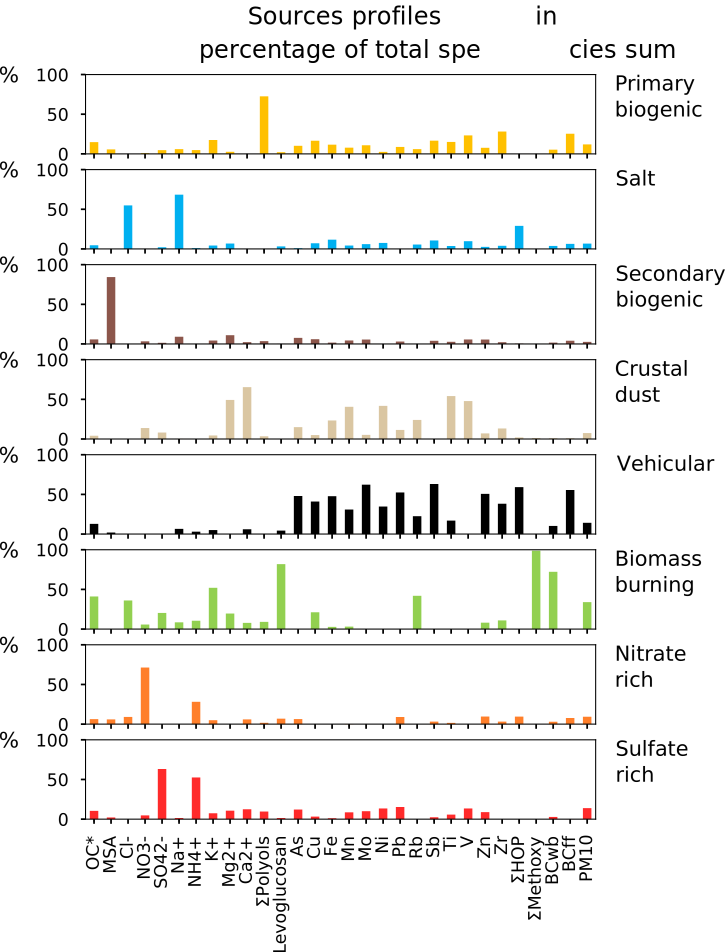
\includegraphics[width=0.8\textwidth]{chapter04/SI_fig01}
%     \caption{Percentage of the ambient species concentration apportioned in each
%         factor attributed by the PMF model.}
%     \label{fig:concPercent}
% \end{figure}
% \clearpage
%
% \subsection{Correlation between OP and chemical species, and OP and
% sources}\label{si-2-correlation-between-op-and-chemical-species-and-op-and-sources}
%
% The univariate correlation on an annual basis between the OP values and the
% concentrations of chemical species was first investigated and is presented in
% Fig.~\ref{fig:pearsonrChem}. We see a strong relationship between some of the
% organic species and the OP (levoglucosan, methoxyphenol) as well as the
% carbonaceous matter (OC and BC) for both tests. It suggests important
% contributions of biomass burning source and fossil fuel burning activities to
% the OP's. The metals Cu, Rb, and Sb appear highly correlated to the OP, but Ni,
% Ti and V do not. The results for the ions indicate weak positive correlations
% with both OP only. We also note that the polyols and MSA show a tendency with
% anti-correlations with both OPs. Most of these results are strongly affected by
% the really high changes in concentrations during the winter and the summer
% periods, in part related to the local impact of meteorology and inversion layers
% in winter \parencite{calasComparison2018}.
%
% \begin{figure}[h]
%     \centering
%     \includegraphics[width=0.7\textwidth]{chapter04/SI_fig02}
%     \caption{Pearson's correlation coefficient between the concentrations of the
%         species and the OP AA\textsubscript{v} and OP DTT\textsubscript{v}
%         activity from the 2, November 2013 to the 31, October 2014 (97 samples).
%         **: p-values \textless{}0.01, *: p-value \textless{}0.05, ns: p-value
%     \textgreater{}0.05.}
%     \label{fig:pearsonrChem}
% \end{figure}
%
% The univariate-correlation between the contributions of the sources of PM
% deduced from the PMF and the OPs is presented Fig.~\ref{fig:pearsonrSrc}. It
% emphasized the hypothesis of the high contribution of the biomass burning and
% vehicular sources to the OP of the PM\textsubscript{10}. We do not see very
% large differences between the two tests, expect for the crustal dust source (no
% correlation with the OP AA\textsubscript{v} but a positive one for the OP
% DTT\textsubscript{v}).
%
% \begin{figure}[h]
%     \centering
%     \includegraphics[width=0.6\textwidth]{chapter04/SI_fig03}
%     \caption{Pearson's correlation coefficient between the PM concentrations of
%         the sources from the PMF and the OP AA\textsubscript{v} and OP
%         DTT\textsubscript{v} activity from the 14, November 2013 to the 31,
%         October 2014 (85 samples). **: p-values \textless{}0.01, *: p-value
%     \textless{}0.05, ns: p-value \textgreater{}0.05.}
%     \label{fig:pearsonrSrc}
% \end{figure}
%
%
%
% \clearpage
%
%
